\section{Metodología y plan de trabajo}

\begin{table}[H]
\centering\footnotesize
\caption{Fases del proyecto.}
\label{tab:fases}
\rowcolors{2}{SoftGray}{white}
\begin{tabularx}{\textwidth}{@{}>{\bfseries\raggedright\arraybackslash}p{3.3cm} >{\raggedright\arraybackslash}X >{\raggedright\arraybackslash}p{4.5cm}@{}}
\toprule
\rowcolor{TableHead} Fase & Qué se hace & Criterio de terminado \\
\midrule
1. Revisión y modelo & Datos publicados, cinco submodelos y simulación de misión & Hecho: este documento \\
2. Núcleo en Verilog & Siete módulos, modelo de referencia, cinco bancos de prueba y prueba en dos DE10-Lite & Hecho: coincidencia total, síntesis sin errores y los cuatro escenarios correctos en las tarjetas \\
3. Sensor y ESP32 & Lectura de la matriz térmica y envío de cuadros por UART & La tarjeta recibe 10 cuadros por segundo sin errores \\
4. Integración & Núcleo en la DE10-Lite con sensor real y con insecto simulado & Detecta una mano a la distancia calculada \\
5. Mediciones & Alcance, falsas alarmas, latencia, recursos y consumo & Tabla de lo medido contra lo calculado \\
6. Insecto vivo (opcional) & Mochila de masa equivalente y estímulo de luz, con el protocolo de la sección~\ref{sec:etica} & Solo con autorización del profesor \\
\bottomrule
\end{tabularx}
\end{table}

\needspace{8\baselineskip}
\textbf{Mediciones previstas y su valor calculado.}
\begin{itemize}
  \item \textbf{Alcance de detección} con una mano y con una cara, a 22~\textdegree C: se esperan 0.9~m para
        confirmar y 1.3~m para empezar a acercarse con la matriz de $8\times8$.
  \item \textbf{Falsas alarmas} con una taza caliente, un foco y la pared asoleada: el criterio de ventana
        debe descartar lo que pase de 38~\textdegree C.
  \item \textbf{Latencia} entre que aparece la mancha y la alerta: ocho cuadros, 0.8~s.
  \item \textbf{Recursos y tiempo}: 722 elementos lógicos y 72~MHz, ya obtenidos; consumo de la tarjeta por medir.
  \item \textbf{Circuito en el lazo}: las mismas misiones de la simulación, con la tarjeta decidiendo los
        estímulos; el resultado debe coincidir con la simulación en software.
\end{itemize}

Si se llega a la fase 6, la plataforma de caminadora esférica con control de temperatura descrita
en~\cite{gracidas2026} permitiría medir el dato que más falta: el ángulo de giro que produce un pulso de
luz ultravioleta de 0.5~s, y cuántos pulsos tolera el insecto antes de habituarse.

\begin{figure}[H]
\centering
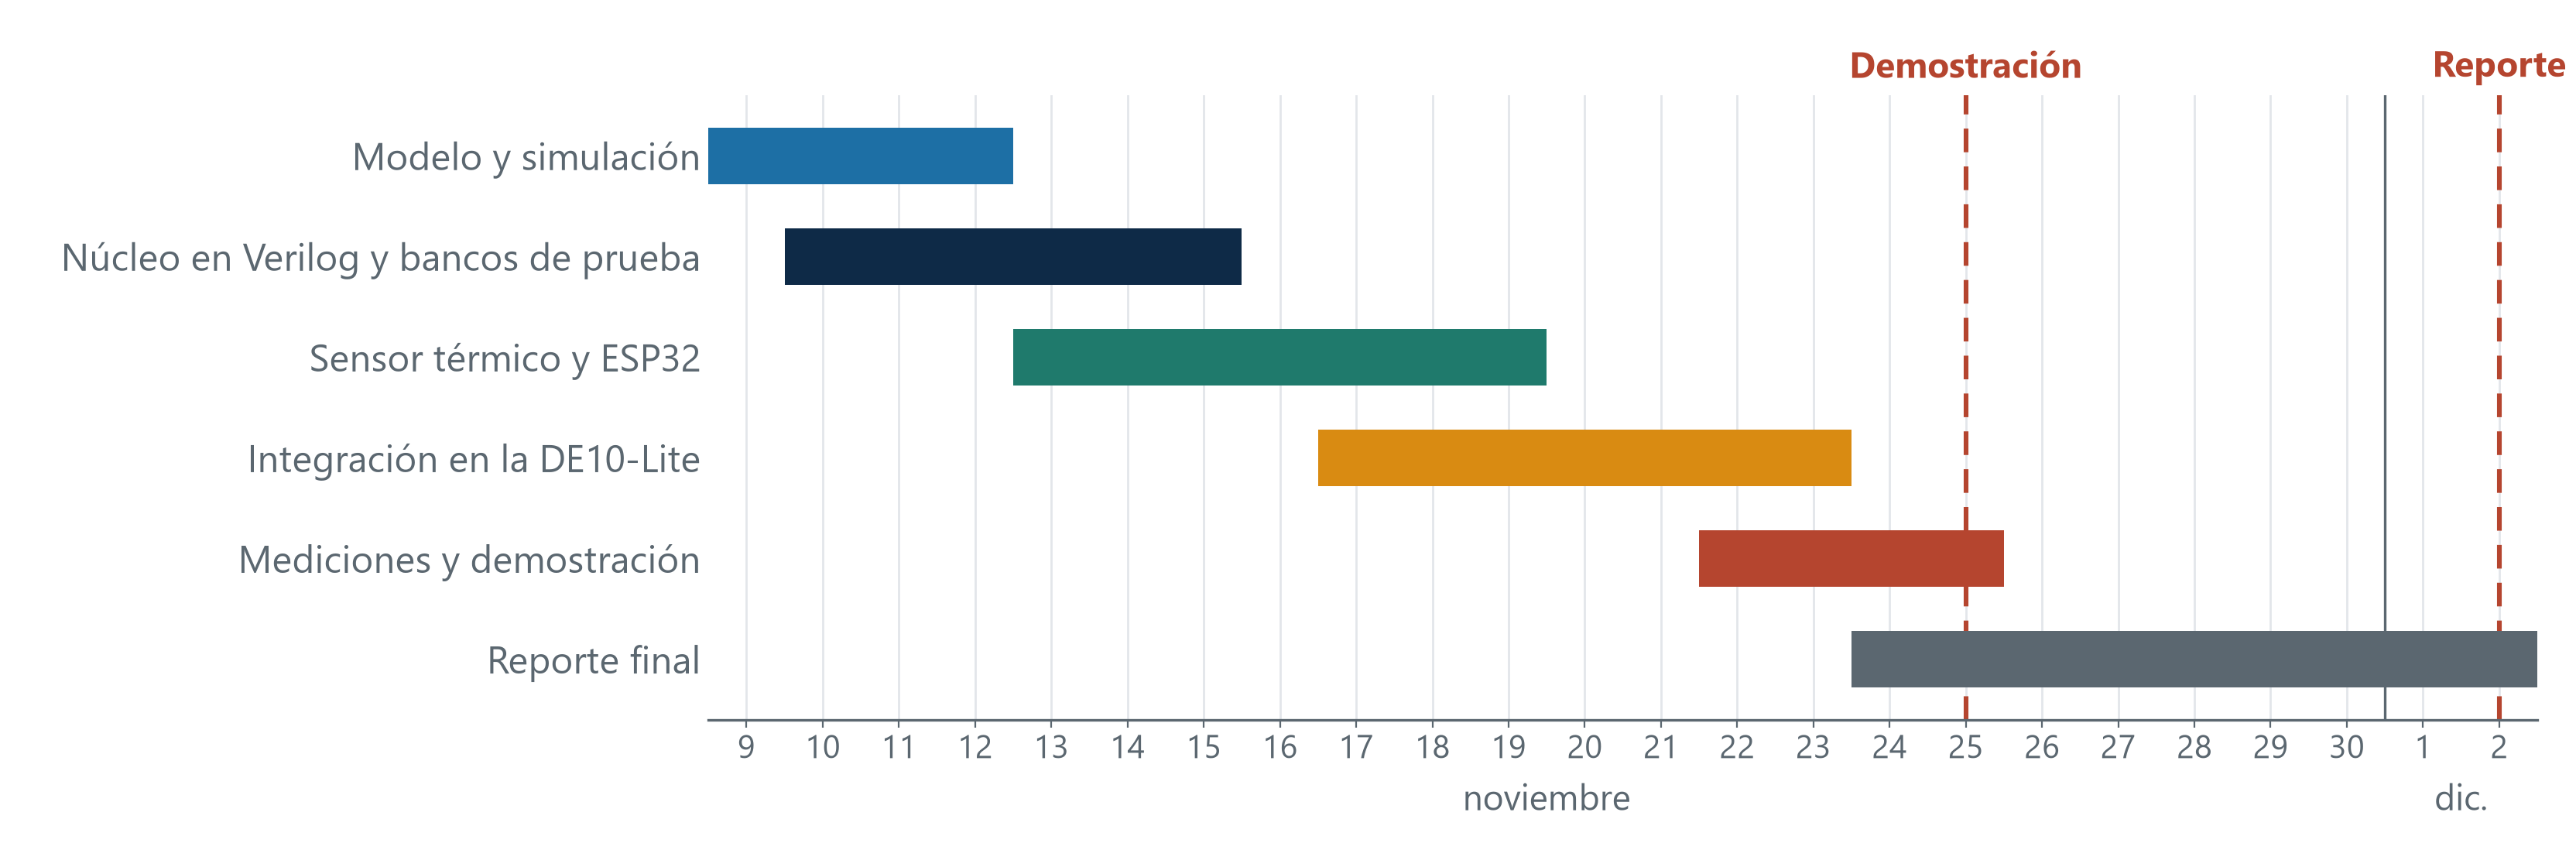
\includegraphics[width=\textwidth]{figs/cronograma.png}
\caption{Cronograma.}
\label{fig:cronograma}
\end{figure}

\needspace{14\baselineskip}
\section{Riesgos y limitaciones}

\begin{table}[H]
\centering\footnotesize
\caption{Riesgos del proyecto y limitaciones del modelo.}
\label{tab:riesgos}
\rowcolors{2}{SoftGray}{white}
\begin{tabularx}{\textwidth}{@{}>{\bfseries\raggedright\arraybackslash}p{4.4cm} >{\raggedright\arraybackslash}X@{}}
\toprule
\rowcolor{TableHead} Riesgo o limitación & Consecuencia y manejo \\
\midrule
La simulación no es un colapso real & Los mapas son sintéticos y en dos dimensiones. Sirve para comparar políticas, no para predecir tiempos de rescate \\
La marcha se midió en arenas iluminadas & No hay datos de marcha a oscuras entre escombro; el análisis de sensibilidad muestra cuánto pesa cada supuesto \\
La respuesta a la luz no está cuantificada & Se usan los valores de electrodos de superficie; la fase 6 lo mediría \\
El ángulo de giro varía de 0 a 110\textdegree{} entre ensayos~\cite{lin2023} & La política no depende de un giro exacto: corrige con el siguiente cuadro \\
La detección falla con ambiente caliente & Límite físico; se documenta y se propone CO$_2$ como señal adicional \\
Recuperar insectos y mochilas está resuelto a medias & En simulación, un refugio y un faro en la entrada recuperan \regFaroDos~\% en dos horas. El faro no se ha medido y siempre queda una parte sin volver; sin esto no hay despliegue responsable \\
La matriz térmica no llega a tiempo & El núcleo se prueba con cuadros que manda una segunda tarjeta por UART, lo que ya funciona en las DE10-Lite \\
La ley exige confinamiento & El proyecto se limita a recinto cerrado \\
\bottomrule
\end{tabularx}
\end{table}

\section{Conclusiones}

\begin{enumerate}
  \item \textbf{El insecto carga menos de lo que se cita.} La meta defendible es una mochila de 2 a 3~g y
        de perfil bajo. La masa del cómputo es despreciable; mandan la batería y el sensor.
  \item \textbf{El estímulo debe ser escaso y sin cirugía.} La luz ultravioleta y los electrodos de superficie
        evitan el implante, y un presupuesto de estímulos acota la habituación con una regla que cabe en
        64 registros.
  \item \textbf{La detección debe contar píxeles, no comparar contra un umbral fijo.} Con una matriz de
        $32\times32$ el acercamiento empieza a 2.5~m y la confirmación ocurre a 1.2~m.
  \item \textbf{El núcleo existe y está verificado.} 477 elementos lógicos y 224 registros, idéntico a su
        modelo de referencia en 11\,424 cuadros, a 72~MHz en la DE10-Lite y con camino a una FPGA de
        2~mg o a un chip propio. En dos tarjetas reales unidas por UART respondió bien a los cuatro
        escenarios: alertó a los 55.1~s con la persona y no alertó en los otros tres.
  \item \textbf{Guiar ayuda, sin milagros.} En la simulación, la política guiada sube la probabilidad de
        detección en una hora de \pPasivaSesenta~\% a \pGuiadaSesenta~\% con diez insectos, y cubre
        \cobGuiada~\% de los huecos frente a \cobPasiva~\%. Diez insectos guiados rinden como entre
        veinte y cuarenta sin guiar. Pesan más el número de insectos y la forma del colapso que la
        política, y girar hacia el calor casi no añade a explorar bien. En uno de los ocho colapsos
        guiar empeora el resultado; un enjambre mixto, mitad guiado y mitad sin estímulos, conserva
        el promedio y evita ese caso.
  \item \textbf{Para que vuelvan hace falta una señal en la entrada.} Esperarlos en un refugio recupera
        \regTrampaDos~\% en dos horas y guiarlos a ciegas, menos. Con un faro que la mochila pueda
        seguir vuelve \regFaroDos~\%. Ningún método los recupera a todos.
  \item \textbf{Los límites son del animal y de la ley.} Temperatura, recuperación y confinamiento definen
        dónde no debe usarse, y decirlo es parte del resultado.
\end{enumerate}

El siguiente paso es la fase 3: conectar la matriz térmica al ESP32 y probar el núcleo con una mano
frente al sensor.
